% !TEX TS-program = Xelatex
% !TEX encoding = UTF-8 Unicode

\documentclass[UTF8]{ctexart}
\usepackage{amsmath}
\usepackage[bottom]{footmisc}
\usepackage{geometry}
\usepackage{graphicx}
\usepackage{hyperref}
\usepackage{figsize}
\usepackage[separate-uncertainty = true,per-mode=symbol]{siunitx}
\usepackage{tabu}
\usepackage{wasysym}
\geometry{left=0.7in,right=0.7in,bottom=0.7in,top=0.7in}
\begin{document}

\title{实验二十三:高温超导材料特性测试和低温温度计}
\author{朱寅杰 1600017721}
\date{2018年6月8日}
\maketitle
\setcounter{section}{23}
\subsection{室温初始数据}
室温下,样品装置放置在桌面上,温差电偶读数为\SI{.013}{\mV}。液面计示数为\SI{.001}{\mV}。标准铂电阻上的电压为\SI{109.67}{\mV},通过的电流为$\SI{100.00}{\mV}/\SI{100}{\ohm}=\SI{1.0000}{mA}$,故其阻值为\SI{109.67}{\ohm},查表得室温为\SI{298.04}{K}。二极管上的电压为\SI{.5062}{\V},通过的电流为$\SI{1.0000}{\V}/\SI{10}{\kilo\ohm}=\SI{.10000}{\mA}$。样品上通过的电流为$\SI{100.217}{\mV}/\SI{10}{\ohm}=\SI{10.0217}{\mA}$,电压为\SI{.226}{\mV},故此时样品电阻为\SI{.02255}{\ohm}。

\subsection{低温温度计比对数据}

\begin{center}
\begin{tabu}{X[c,-10]X[c,-10]X[c,-10]X[c,-10]||X[c,-10]X[c,-10]X[c,-10]}
\hline
铂电阻压降/mV&温度/K&二极管压降/V&二极管电阻/\si{k\ohm}&铂电阻压降/mV&温度/K&温差电偶压降/mV\\
\hline
108.94 &296.13 &0.5122 &5.122 &108.67 &295.44 &5.972
\\102.58 &279.79 &0.5495 &5.495 &102.28 &279.02 &5.365
\\96.35 &263.89 &0.5870 &5.870 &96.07 &263.18 &4.786
\\89.59 &246.74 &0.6293 &6.293 &89.25 &245.88 &4.189
\\84.50 &233.88 &0.6610 &6.610 &84.23 &233.20 &3.756
\\78.90 &219.79 &0.6989 &6.989 &78.45 &218.66 &3.292
\\70.25 &198.15 &0.7496 &7.496 &69.96 &197.42 &2.655
\\65.10 &185.34 &0.7802 &7.802 &64.59 &184.08 &2.280
\\61.65 &176.80 &0.8003 &8.003 &61.38 &176.14 &2.064
\\57.78 &167.27 &0.8235 &8.235 &57.54 &166.68 &1.802
\\54.27 &158.66 &0.8438 &8.438 &54.96 &160.35 &1.582
\\51.05 &150.79 &0.8619 &8.619 &50.85 &150.31 &1.401
\\47.55 &142.29 &0.8814 &8.814 &47.36 &141.83 &1.207
\\45.20 &136.60 &0.8944 &8.944 &44.95 &136.00 &1.074
\\43.54 &132.60 &0.9028 &9.028 &43.37 &132.19 &0.996
\\40.70 &125.77 &0.9180 &9.180 &40.30 &124.81 &0.820
\\37.65 &118.47 &0.9340 &9.340 &37.32 &117.69 &0.680
\\34.20 &110.26 &0.9520 &9.520 &33.94 &109.64 &0.526
\\31.37 &103.55 &0.9652 &9.652 &31.20 &103.15 &0.413
\\30.67 &101.89 &0.9690 &9.690 &30.48 &101.44 &0.382
\\
\hline
\end{tabu}
\end{center}
作图及分析见附页。


\subsection{样品电阻随温度的变化}
\begin{center}
\begin{tabu}{X[c,-10]X[c,-10]X[c,-10]X[c,-10]||X[c,-10]X[c,-10]X[c,-10]X[c,-10]}
\hline
Pt电阻压降/mV&温度/K&样品压降/mV&样品电阻/\si{m\ohm}&Pt电阻压降/mV&温度/K&样品压降/mV&样品电阻/\si{m\ohm}\\
\hline
108.44&294.81&0.224&22.35&28.92&97.73&0.097&9.68 \\
101.80&277.76&0.213&21.25&28.48&96.69&0.096&9.58 \\
95.75&262.34&0.202&20.16&28.32&96.32&0.095&9.48 \\
88.88&244.91&0.191&19.06&27.95&95.45&0.094&9.38 \\
83.90&232.34&0.183&18.26&27.82&95.14&0.093&9.28 \\
77.88&217.20&0.174&17.36&27.69&94.83&0.092&9.18 \\
69.48&196.20&0.162&16.16&27.35&94.03&0.090&8.98 \\
64.32&183.38&0.154&15.37&27.12&93.49&0.087&8.68 \\
61.05&175.29&0.150&14.97&26.92&93.02&0.084&8.38 \\
57.15&165.69&0.146&14.57&26.75&92.62&0.081&8.08 \\
53.55&156.87&0.140&13.97&26.60&92.27&0.076&7.58 \\
50.58&149.62&0.138&13.77&26.54&92.13&0.070&6.98 \\
47.18&141.36&0.132&13.17&26.50&92.03&0.065&6.49 \\
44.68&135.32&0.128&12.77&26.42&91.84&0.049&4.89 \\
39.98&124.02&0.123&12.27&26.37&91.73&0.029&2.89 \\
36.88&116.61&0.116&11.57&26.33&91.63&0.017&1.70 \\
33.68&108.99&0.111&11.08&26.20&91.33&0.014&1.40 \\
31.03&102.71&0.105&10.48&25.97&90.79&0.013&1.30 \\
30.37&101.15&0.108&10.78&25.59&89.89&0.012&1.20 \\
29.87&99.97&0.111&11.08&24.11&86.42&0.012&1.20 \\
29.47&99.03&0.100&9.98&			\\
\hline
\end{tabu}
\end{center}
前18个数据点(102K~295K)用软件去作电阻值与温度的线性拟合,得到截距为\SI{4.66(13)}{m\ohm},斜率为\SI{.05926(66)}{m\ohm/K},相关系数为\num{.99902}。从样品电阻行为开始偏离直线的位置看,起始转变温度约在\SI{101}{K}左右。当样品上的压降减小到\SI{.017}{mV}时,将电流反相,电压表示数不变,证明此时的电压已经全是杂散电动势的贡献,故认为零电阻温度在\SI{91.6}{\K}左右。将坐标轴移动到\SI{1.7}{m\ohm}处,把拟合的直线除以二,与样品电阻的实际行为相交,得到转变中点温度约为\SI{91.9}{\K}。
\begin{figure}
  \centering
  \includegraphics[width=0.8\linewidth]{wdj.eps}
  \caption{图示为热电偶电压和(在0.1mA下工作的)硅管的电阻随温度变化的曲线。温度值使用铂电阻对表算出。可以看到在100K~300K段,硅管的电阻与温度呈负相关,而温差电偶的电压与温度呈正相关。二者在局部线性都较好,要求不高时可以当低温温度计使。}
  
  \includegraphics[width=\linewidth]{trans.eps}
  \caption{图示为样品电阻随温度的变化,102K~295K段作了线性拟合。}
\end{figure}
\subsection{浸没入液氮中的检测数据}
直接把整个装置浸没入液氮里,
铂电阻上的电压为\SI{20.29}{\mV},通过的电流为$\SI{99.88}{\mV}/\SI{100}{\ohm}=\SI{.9988}{\mA}$,比测量开始时变化了千分之一,认为铂电阻上的电流保持基本稳定。此时铂电阻的阻值为\SI{20.31}{\ohm},对应的温度为\SI{77.54}{\K}。液面计和温差电偶的示数均为\SI{.000}{\mV},符合预期。通过硅二极管的电流为$\SI{1.0004}{\V}/\SI{10}{\kilo\ohm}=\SI{.10004}{\mA}$,两端电压为\SI{1.0212}{\mV},电流与开始时相比只变化了万分之四。样品两端电压为\SI{.018}{\mV},通过样品的电流为$\SI{100.206}{mV}/\SI{10}{\ohm}=\SI{10.0206}{mA}$。电流与开始时相比变化了百分之二,尚可以接受。电流反向后电压示数不变,证明电压示数全是杂散电动势的贡献。从中可见我们测量得到的数据基本都是靠谱的。

\end{document} 